\documentclass[paper=a4, 12pt]{report}

\usepackage[margin=0.9in]{geometry} % margin size

% choose language and encoding options
\usepackage[frenchb]{babel}
% \usepackage[english]{babel}  % decomment to use English
\usepackage[utf8]{inputenc}

% some useful options for tables and arrays
\usepackage{booktabs}
\usepackage{array}
\newcolumntype{L}[1]{>{\raggedright\let\newline\\\arraybackslash\hspace{0pt}}m{#1}}
\newcolumntype{C}[1]{>{\centering\let\newline\\\arraybackslash\hspace{0pt}}m{#1}}
\newcolumntype{R}[1]{>{\raggedleft\let\newline\\\arraybackslash\hspace{0pt}}m{#1}}

% fonts
\usepackage{libertine}

% custom colors - you can define your own colours
\usepackage{color}
\definecolor{deepblue}{rgb}{0,0,0.5}
\definecolor{deepred}{rgb}{0.6,0,0}
\definecolor{deepgreen}{rgb}{0,0.5,0}

% maths
\usepackage{amsmath}

% misc
\usepackage{url}

% page formating with the "fancy header" package
\usepackage{sectsty} % Allows customising section commands
\usepackage{fancyhdr} % Custom headers and footers
\pagestyle{fancyplain} % Makes all pages in the document conform to the custom headers and footers
\fancyhead{} % header
\fancyfoot[L]{} % left footer
\fancyfoot[C]{\thepage} % centre footer
\fancyfoot[R]{}  % right footer
\renewcommand{\headrulewidth}{1pt} 
\renewcommand{\footrulewidth}{1pt} 
\setlength{\headheight}{13.6pt} % Customize the height of the header

\usepackage{lipsum} % generate dummy text
\usepackage{amsmath,amsfonts,amsthm} % maths packages
\usepackage{graphicx} % graphics package


%%%%%%%%%%%%%%%%%%%%%%%%%%%%%%%%%%%%%%
 % Le contenu de votre document commence ici
%%%%%%%%%%%%%%%%%%%%%%%%%%%%%%%%%%%%%%

\begin{document}

\title{Rapport projet Traitement Automatique des Langues}
\author{Florent VOLLMER - Thibaut WITCZAK}
\date{05 Mai 2018}
\maketitle

\section{Introduction}
\vspace{0.5cm}
Bob est un chatbot conspirationniste : Il croit à diverses théories du complot. Quelque soit le sujet de la conversation, il essaiera de l’orienter vers une de ces théories, afin d’exposer son point de vue à l’utilisateur. Il montre une attitude sceptique, voire condescendante, face aux réponses de l’utilisateur, qu’il juge “trop formatées”.

\vspace{0.5cm}

Il peut également paniquer si il pense que l’utilisateur est au centre d’une de ces théories (par exemple s’il croit être face à un reptilien), ou quitter la conversation si il s’ennuie (car on ne parle pas assez de sujet qui l’intéressent) ou encore si il trouve l’utilisateur trop “contrariant”, ne croyant pas à ses théories.

\vspace{0.5cm}

Nous l’avons codé anglophone, principalement pour éviter d’avoir affaire à une grammaire trop complexe, introduisant trop de pièges que nous aurions eu à éviter pour pouvoir espérer arriver à des résultats concluants.

\section{Objectif du projet et motivations}
\vspace{0.5cm}
Notre but en choisissant ce thème n’est pas de propager des théories du complots, mais au contraire de les tourner en dérision en les faisant défendre par un programme qui ne “comprend” pas vraiment ce qu’il dit. On a aussi pensé que ce thème serait amusant et donnerait lieu à des conversations atypiques avec l’utilisateur.


\vspace{0.5cm}

Cela a également amélioré nos compétences en Python et nous a appris le Latex. Nous n’avons en revanche pas eu beaucoup d’informations sur ce qui est considéré comme de “bonnes pratiques” en Python, et avons seulement une meilleure idée de comment faire du code fonctionnel dans ce langage.


\vspace{0.5cm}

Enfin, ce projet nous aura enfin permis de nous intéresser à un nouveau type de programme, en appliquant ce que nous avons vu en cours mais aussi en nous laissant une certaine liberté, aussi bien dans le thème de chatbot que dans son fonctionnement.


\section{Fonctionnement du projet}
\vspace{0.5cm}
Répartition du code dans les fichiers :

\vspace{0.5cm}

\textbf{Main.py :} \\
Sert d’interface entre l’utilisateur et Bob

\vspace{0.5cm}

\textbf{Bob :} \\
Regroupe toutes les fonctionnalités propres à Bob, telles que les modes 1, 2 et 3, ou encore la gestion des émotions.

\vspace{0.5cm}

\textbf{LexField :} \\
Regroupe tout ce qui touche à la gestion des champs lexicaux : reconnaître si un mot y appartient, fournir des réponses génériques… Les champs lexicaux sont regroupés en fichiers, contenant à la fois les mots, les groupes de mots, les réponses, les “influences” sur Bob et les liens avec les autres champs. Un mot peut faire partie de plusieurs champs lexicaux, mais on préfère généralement le mettre dans un minimum de champs lexicaux puis utiliser les liens de parenté. 

\vspace{0.5cm}

\textbf{Answer :} \\
Consistant en une chaîne et un ID, a été créée pour rendre le code plus maintenable. En effet, quand on modifie un détail de formulation ou d’orthographe dans une réponse, pas besoin de la modifier partout : seul son ID est comparé avec celui d’autres réponses.


\vspace{0.5cm}

\textbf{Fichiers texte :} \\
Ces fichiers contiennent des listes de champ lexicaux. LexFields.txt est celui utilisé par le mode2, c’est le plus lourd et le plus générique. Les autres fichiers contiennent des mots-clés et des réponses qui ont un sens seulement dans certains contextes, identifiés dans le mode 3.

\vspace{0.5cm}

Comme demandé, le code a été organisé en 3 modes, correspondant aux méthodes ansBob1, ansBob2 et ansBob3.

\vspace{0.5cm}

\textbf{Mode 1 :} \\
Bob  envoie des réponses comme “hmm…” ou “interesting…”, laissant penser qu’il prête attention à ce que l’utilisateur dit.

\vspace{0.5cm}

\textbf{Mode 2 :} \\
Bob se sert d’un tableau “subjects”, contenant une valeur réelle positive pour chaque sujet de conversation possible. La plus haute de ces valeurs correspond au sujet que Bob estime être le plus pertinent, en fonction des mots entrés par l’utilisateur dernièrement. Il pose ainsi des questions ou fait des remarques sur ces sujets afin d’alimenter la conversation, à la façon d’Elizia, à part que ses répliques ne visent pas à faire parler l’utilisateur de lui, mais de ce qu’il pense sur divers sujets.

\vspace{0.5cm}

Une autre différence avec Elizia est que les valeurs du tableau “subjects” ne sont pas remises à 0 à chaque réponse, mais sont multipliées par 0,6 et remises à 0 seulement si le résultat est en-dessous de 0,4. Cela fait qu’il restera une trace d’un sujet abordé pendant au moins 1 tour dans le tableau (et plus si on a insisté sur le sujet), ce qui permet de ne pas retomber immédiatement dans le mode 1 si l’utilisateur n’a pas entré de mot clé reconnu dans sa dernière réponse.

\vspace{0.5cm}

Enfin, certains des sujets ont des “parents”, qui sont incrémentés de 0,6*value quand le sujet de base est incrémenté de value. Cela ne suffit donc pas à donner la priorité au sujet parent car ce n’est pas ce qu’on recherche, mais en cumulant plusieurs sujets qui ont le même parent, le parent peut effectivement devenir le sujet le plus pertinent.

\vspace{0.5cm}

\textbf{Mode 3 :} \\
On vérifie un ensemble de critères sur le tableau “subjects”, mais aussi sur l’humeur de Bob et on fait des vérifications plus précises sur la dernière phrase entrée par l’utilisateur. On prend également en compte la dernière question posée par Bob, afin qu’il sache que l’utilisateur répondait à l’une de ses questions. Il peut alors envoyer des phrases plus cohérentes avec le contexte.

\vspace{0.5cm}

Pour analyser au mieux la dernière phrase de l’utilisateur, on a codé les méthodes checkStunned et checkYesNo de Bob. Ces méthodes font ce que fait le mode 2 mais de façon plus précise et plus au cas par cas, en utilisant notamment des poids pour chaque mot ou groupe de mot. Ces fonctions sont appelées occasionnellement par le mode 3 suite à certaines questions de Bob :

\vspace{0.5cm}

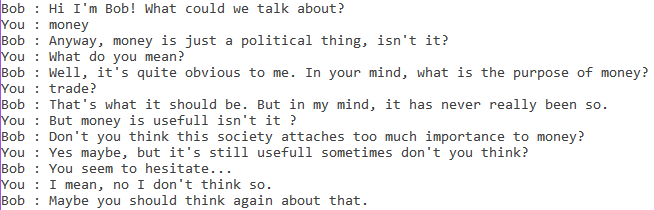
\includegraphics[scale=0.5]{screen1.png}

\vspace{0.5cm}

Ici, Bob a commencé par une réponse de mode 2 car le sujet money l’intéresse mais les conditions n’étaient pas remplies pour entrer en mode 3. En revanche, “Anyway, money is just a political thing, isn’t it?” Est une des questions de Bob dont le mode 3 va analyser la réponse. Ici il a remarqué que l’utilisateur avait l’air surpris, il a alors enchaîné sur une autre question, afin de préciser son propos. Cette question “What is the purpose of money?” est également traitée par le mode 3, mais cette fois en faisant appel à une méthode appelée “miniMode2”, car elle fait elle-même appel au mode 2, mais en lui fournissant une liste de champs lexicaux contenant des mot-clés et des réponses autres que ceux par défaut.

\vspace{0.5cm}

Après avoir donné son avis à l’utilisateur sur sa réponse à l’utilité de l’argent, Bob est sorti du mode 3. Mais comme l’utilisateur a continué à parler d’argent, il lui posé une autre question de mode 2, qui en l’occurrence menait également au mode 3 (“Don’t you think this society attaches too much importance to money?”) . La réponse à cette question a été analysée par la méthode checkYesNo. Malgré la présence du mot “yes”, Celle-ci a considéré que l’utilisateur n’était pas assez clair, la méthode “askYesNo” a donc été appelée pour lui demander d’être plus clair (Elle n’aurait pas été appelée une deuxième une deuxième fois si l’utilisateur avait encore hésité, afin de ne pas bloquer la conversation). La deuxième réponse a été considérée comme un “non”, Bob a alors montré sa désapprobation via la méthode “disapprove”.

\vspace{0.5cm}

L’humeur de Bob est codée sur 3 entiers, qui sont son intérêt pour la conversation, son stress et sa sympathie pour l’utilisateur.

\vspace{0.5cm}

L’intérêt est initialisé avec une valeur de 0, est décrémenté à chaque fois que le mode 1 est employé, et est remis à 0 à chaque fois que les modes 2 ou 3 sont employés. Si l’intérêt de Bob atteint la valeur -5, il quitte la conversation comme ci-dessous :

\vspace{0.5cm}

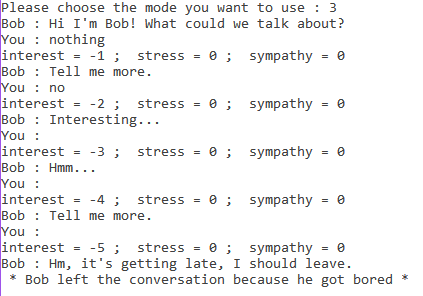
\includegraphics[scale=0.5]{screen2.png}

\vspace{0.5cm}

Dans cet exemple, on n’est jamais sorti du mode 1, alors que le mode 3 était activé. Bob a donc vite perdu patience.

\vspace{0.5cm}

Le stress est initialisé à 0, et peut être augmenté via le mode 2 ou le mode 3, à cause de certains mot clés (les questions sur lui, et les agences de renseignement parce qu’il est persuadé d’être traqué par celles-ci) ou des réponses de l’utilisateur à certaines questions. Si Bob est trop stressé, il fuira la conversation comme dans les deux cas ci-dessous :

\vspace{0.5cm}

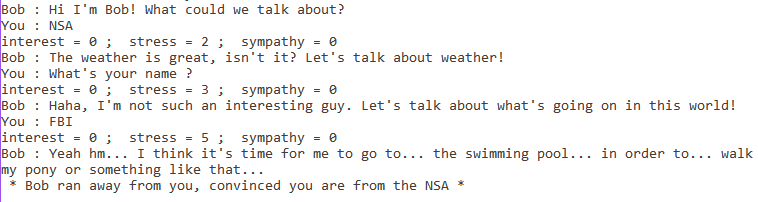
\includegraphics[scale=0.5]{screen3.png}

\vspace{0.5cm}

Ici Bob a d’abord été stressé par le mot NSA. C’est le mode 2 qui est intervenu, aussi bien pour monter l’attribut stress que pour fournir la réponse de Bob, qui cherche à détourner la conversation. Il s’est passé la même chose quand l’utilisateur lui a demandé son nom. Quand on a enchaîné sur le mot FBI, le mode 2 a encore incrémenté le stress de 2 points, ce qui a déclenché la fuite de Bob, qui a trouvé un prétexte douteux pour s’en aller.

\vspace{0.5cm}

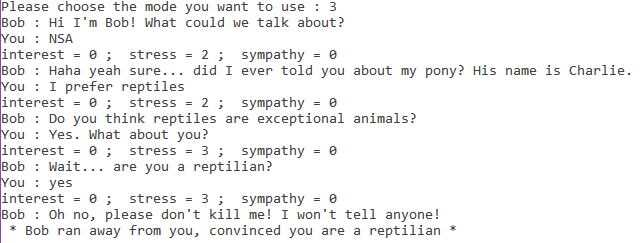
\includegraphics[scale=0.5]{screen4.png}

\vspace{0.5cm}

Dans cet autre exemple, Bob a également été stressé par les questions sur lui et par le mot NSA, mais cette fois le tableau “subjects” indiquait qu’on l’on parlait aussi de reptiles. Bob a donc vu un lien avec les reptiliens, et a demandé à l’utilisateur si il en était un. Lorsque celui-ci a répondu par l’affirmative, Bob a également pris la fuite.

\vspace{0.5cm}

Enfin, il est possible de contrarier Bob suffisamment pour qu’il quitte de lui-même la conversation. En effet, il aime qu’on soit d’accord avec lui, et ne voudra plus vous parler si son attribut sympathie atteint la valeur -5 ou en dessous. Cette variable est initialisée à 0, et peut être incrémentée ou décrémentée selon les réponses de l’utilisateur. Il est techniquement possible de la faire baisser directement via le mode 2, mais dans le projet seul le mode 3 la modifie, parfois via le mode 2 appelé par la méthode miniMode2 (on est donc toujours en mode 3).

\vspace{0.5cm}

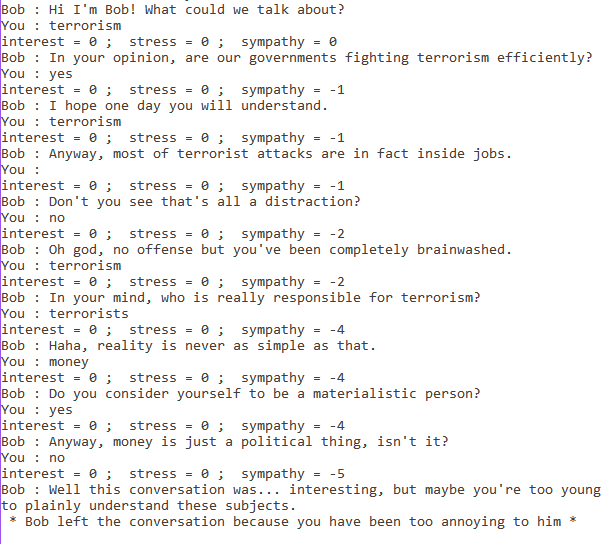
\includegraphics[scale=0.5]{screen5.png}

\vspace{0.5cm}

Ici Bob n’a pas été content parce que l’utilisateur a toujours répondu une des “pires” réponses possibles à chaque question de Bob, aussi bien sur le terrorisme que sur l’argent. Bien que les variables affichées ici sont normalement masquées, L’utilisateur peut deviner s’il gagne la sympathie de Bob ou non en regardant les réponses fournie par le mode 3, plus précisément par “miniMode2” (“Haha, reality is never as simple as that”) ou par les méthodes “Approve” et
“Disapprove” (“Oh god, no offense but you’ve been completely brainwashed”, “I hope one day you will understand”). Ces réponses sont ici toutes très condescendantes, mais peuvent être plus amicales quand il faut montrer que la sympathie de Bob augmente.

\section{Limites et améliorations possibles du projet}
\vspace{0.5cm}
Nous avons choisi de faire un chatbot axé sur les champs lexicaux, et non pas sur la grammaire et les constructions de phrases. Bob est donc incapable de reconnaître des choses trop compliquées, telles que des doubles négations. Il ne sait pas non plus construire ses propres phrases, et pioche toujours parmis une liste de phrases toutes faites.

\vspace{0.5cm}

De plus, le nombre de théories et de champs lexicaux que Bob connaît est relativement limité, ainsi même le mode 2, censé être relativement robuste, ne trouve souvent rien de particulier à dire sur la phrase entrée par l’utilisateur, et on doit faire appel au mode 1. Une amélioration possible serait d’agrandir lesdits champs lexicaux et d’augmenter leur nombre en faisant plus de recherches sur les différentes théories.

\vspace{0.5cm}

On pourrait aussi générer les champs lexicaux automatiquement en analysant plusieurs articles sur différents sujets, et donner un “poids” à chaque mot ou groupe de mots pour chaque catégorie, correspondant à sa fréquence d’apparition dans ce sujet, à la manière de l’exercice sur la détection de spam fait en classe, et ainsi avoir une analyse à la fois plus fine et plus robuste.

\vspace{0.5cm}

Si l’on voulait mettre en application les améliorations précédemment citées, on pourrait rencontrer des problèmes de performances et il faudrait alors sans doute revoir la structure des fichiers et des données, afin d’avoir quelque chose de plus optimisé. Par exemple, on pourrait stocker tous les mots et groupes de mots par ordre alphabétique afin de vérifier plus rapidement s’ils existent dans au moins 1 champ lexical, puis d’accéder à une liste de nombres correspondant à leurs poids dans différents sujets. Dans le cas du mot “sugar” par exemple, on chercherait “sugar” par bijection dans une unique liste de mots, et une fois trouvé on incrémenterait la pertinence du sujet “alimentation” de 10, celle de “addiction” de 7, et celle de “IT” de 1 (pour “syntactic sugar”). On vérifierait également s’il fait partie d’un quelconque groupe de mots, pour lesquels il faudrait trouver une solution.

\vspace{0.5cm}

Il y a sans doute également des progrès à faire dans les relations entre les champs lexicaux. Pour cela il faudrait trouver un compromis entre la “réalité” analysée dans des articles de presse par exemple, et le caractère complotiste de Bob, qui va voir des liens là où le commun des mortels n’en voit pas.

\vspace{0.5cm}

Une autre limite de Bob est l’aspect un peu brouillon du mode 3, qui ne supporterait sans doute pas d’être complexifié beaucoup plus. Il faudrait donc trouver un moyen de rendre son code plus générique, et de mettre les variantes au cas par cas dans des fichiers .txt ou .csv par exemple, qui pourraient être bien plus nombreux et seraient lus par le mode 3, un peu à la manière des fichiers de champs lexicaux lus par le mode 2.

\section{Contributions des membres au projet}
\vspace{0.5cm}
Florent a essentiellement contribué au développement du code du chatbot. Ainsi, il aura davantage travaillé sur les modes 2 et 3 du programme.

\vspace{0.5cm}

Thibaut, quant à lui, a créé le mode 1 et a contribué au code au début du projet.
Il s’est ensuite principalement occupé du rapport et de la maîtrise du latex, et a grandement participé au contenu des fichiers de champs lexicaux.

\end{document}